\chapter{المول والكتلة المولية}\label{ch:g10:the-mole}

في نهاية اليوم لا يعدّ المصرف قطعه النقدية قطعةً قطعة: بل يزنها. فإذا كانت
كتلة القطعة الواحدة \qty{7.5}{g}، فإن كيسًا من القطع كتلته \qty{7.5}{kg}
يحوي ألف قطعة، ويكون الميزان قد قام بالعدّ. ويواجه الكيميائيون المشكلة نفسها
مع \omterm{def:g7:atoms-and-molecules:atom}{الذرات}، لكنها أسوأ بكثير: فملعقة من الماء تحوي من \omterm{def:g7:atoms-and-molecules:molecule}{الجزيئات} أكثر مما على
شواطئ ساحل كامل من حبات الرمل. ويحلّونها بالطريقة نفسها، بالوزن، والكيس
الذي يستعملونه يحوي
\num{602214076000000000000000} كيان. يعرّف هذا الفصل ذلك الكيس، أي
\omterm{def:g10:the-mole:amount}{المول}، ويبيّن كيف ننتقل من كتلة على الميزان إلى عدد من \omterm{def:g7:atoms-and-molecules:atom}{الذرات} أو
\omterm{def:g7:atoms-and-molecules:molecule}{الجزيئات}.

\begin{recall}
كتلة \omterm{def:g7:atoms-and-molecules:atom}{الذرة} متركزة في نواتها؛ وكتلة كل من \omterm{def:g9:inside-the-atom:proton}{البروتون} \omterm{def:g9:inside-the-atom:proton}{والنيوترون} نحو
\qty{1.67e-27}{kg}، فكتلة \omterm{def:g7:atoms-and-molecules:atom}{ذرة} عددها الكتلي $A$ نحو
$A \times \qty{1.67e-27}{kg}$. وتُكتب الأعداد الكبيرة والصغيرة بالكتابة
العلمية (\cref{ch:g9:inside-the-atom}). \omterm{def:g7:atoms-and-molecules:formula}{والصيغة الكيميائية} تعطي عدد \omterm{def:g7:atoms-and-molecules:atom}{ذرات} كل
عنصر في \omterm{def:g7:atoms-and-molecules:molecule}{الجزيء} (\cref{ch:g7:atoms-and-molecules}).
\end{recall}

\begin{omfigure}
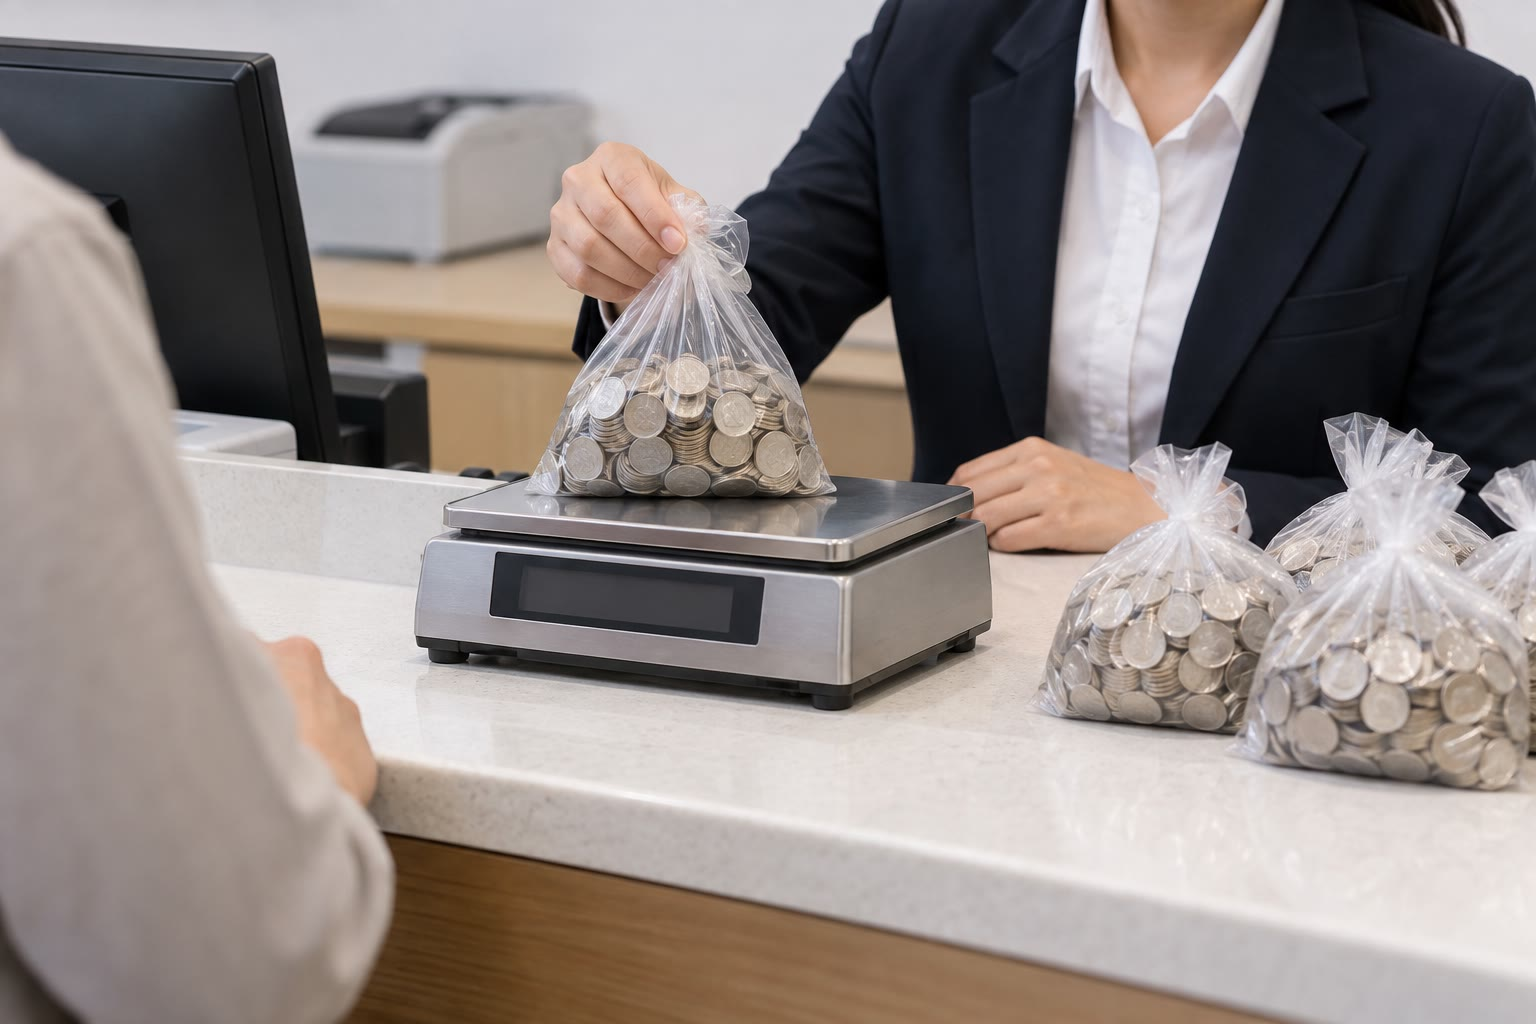
\includegraphics[width=0.55\linewidth]{images/book1/ai/g10-bank-coins.jpg}

{\small المصرف يعدّ القطع النقدية بوزنها. والكيميائيون يعدّون \omterm{def:g7:atoms-and-molecules:atom}{الذرات} بالطريقة
نفسها.}
\end{omfigure}

\section{العدّ بالوزن}

\begin{example}[كيس من القطع النقدية]\label{ex:g10:the-mole:coins}
كتلة القطعة النقدية \qty{7.5}{g}. وكتلة كيس من هذه القطع
\qty{1.80}{kg}، أي \qty{1800}{g}، دون حساب كتلة الكيس نفسه. فهو
يحوي
\[
  \frac{\qty{1800}{g}}{\qty{7.5}{g}} = 240 \text{ قطعة.}
\]
وللعدّ يقسم المصرف الكتلة الكلية على كتلة قطعة واحدة.
\end{example}

\begin{example}[ملعقة من الماء]\label{ex:g10:the-mole:spoon}
\omterm{def:g7:atoms-and-molecules:molecule}{لجزيء} الماء، \ce{H2O}، $2 + 16 = 18$ نوكليونًا (\omterm{def:g7:atoms-and-molecules:atom}{فذرات} الأكسجين 16
والهيدروجين 1 تكاد تكوّن الماء الطبيعي كله)، فكتلته نحو
$18 \times \qty{1.67e-27}{kg} = \qty{3.0e-26}{kg}$، أي
\qty{3.0e-23}{g}. ولذلك فملعقة فيها \qty{5.0}{g} من الماء تحوي
\[
  \frac{\qty{5.0}{g}}{\qty{3.0e-23}{g}} \approx \num{1.7e23}
  \text{ جزيء.}
\]
تجري القسمة كما في القطع النقدية، لكن الجواب عدد لا يستطيع أحد أن يتصوره.
فالكيميائيون يحتاجون إلى رزمة من \omterm{def:g7:atoms-and-molecules:atom}{الذرات} تناسب عيّنات
المختبر.
\end{example}

\begin{definition}[كمية المادة والمول]\label{def:g10:the-mole:amount}
% ledger: const:NA
\emph{كمية المادة}\index{كمية مادة} $n$ في عيّنة تعدّ الكيانات التي تحويها
(\omterm{def:g7:atoms-and-molecules:atom}{ذرات}، أو \omterm{def:g7:atoms-and-molecules:molecule}{جزيئات}، أو \omterm{def:g9:ions:ion}{أيونات}، يُذكر نوعها في كل مرة). ووحدتها
\emph{المول}\index{مول}، ورمزه \si{mol}: والمول الواحد يحوي
\num{6.02214076e23} كيانًا بالضبط.
\end{definition}

\begin{remark}[الدزينة والرزمة والمول]\label{rem:g10:the-mole:dozen}
\omterm{def:g10:the-mole:amount}{المول} وحدة عدّ، مثل دزينة البيض (12) أو رزمة الورق (500 ورقة)، لكنه أكبر
بكثير جدًا. فعبارة «مولان من \omterm{def:g7:atoms-and-molecules:molecule}{جزيئات} الماء» تعني
$2 \times \num{6.02214076e23} = \num{1.20e24}$ \omterm{def:g7:atoms-and-molecules:molecule}{جزيء}، كما تعني عبارة
«دزينتان من البيض» 24 بيضة. واذكر دائمًا الكيانات المعدودة: \omterm{def:g10:the-mole:amount}{فمول} واحد من
\emph{\omterm{def:g7:atoms-and-molecules:molecule}{جزيئات}} الأكسجين \ce{O2} يحوي مولين من
\emph{\omterm{def:g7:atoms-and-molecules:atom}{ذرات}} الأكسجين.
\end{remark}

\begin{history}[فرضية أفوغادرو، 1811]
اقترح الفيزيائي أميديو أفوغادرو سنة 1811 أن الأحجام المتساوية من غازات مختلفة،
في درجة الحرارة والضغط نفسيهما، تحوي العدد نفسه من الجسيمات. وفهم أيضًا أن
غازًا مثل الأكسجين مكوّن من \omterm{def:g7:atoms-and-molecules:molecule}{جزيئات} ثنائية \omterm{def:g7:atoms-and-molecules:atom}{الذرة}. وأُهملت فكرته نحو خمسين سنة،
حتى استعملها ستانيسلاو كانيتسارو سنة 1860 للحصول على مجموعة متسقة من الأوزان
الذرية. وسُمّي الثابت الذي يعدّ كيانات \omterm{def:g10:the-mole:amount}{المول} لاحقًا باسم أفوغادرو؛ ولم يعرف
هو قيمته قط.
\end{history}

\begin{omfigure}
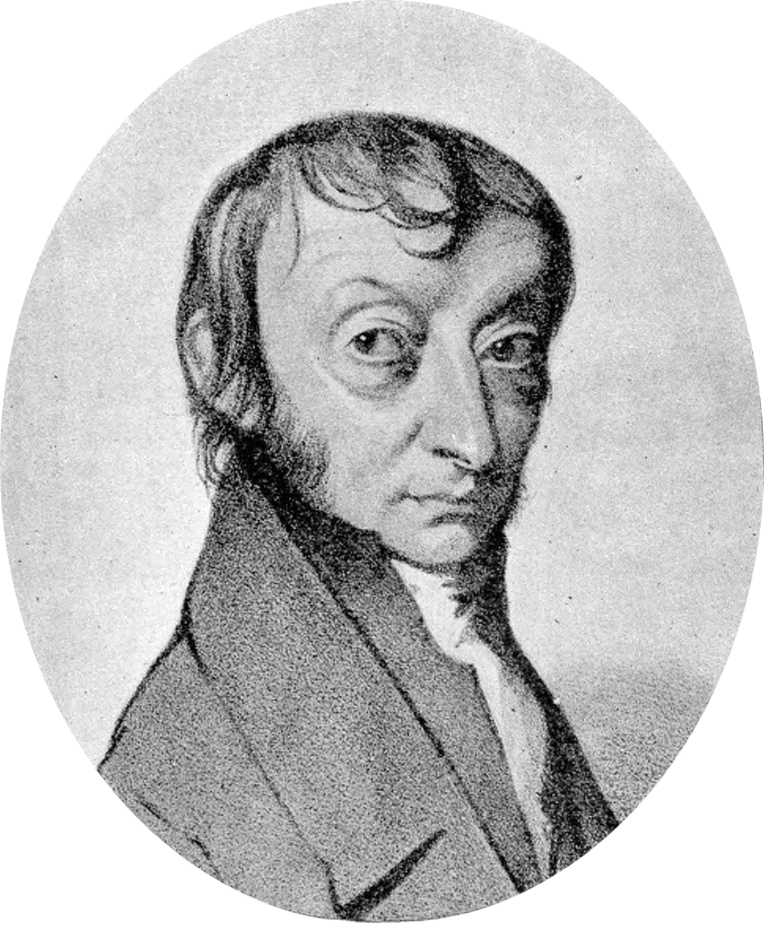
\includegraphics[width=0.26\linewidth]{images/book1/avogadro.jpg}

{\small أميديو أفوغادرو (1776--1856).}
\end{omfigure}

\section{ثابت أفوغادرو}

\begin{definition}[ثابت أفوغادرو]\label{def:g10:the-mole:avogadro}
% ledger: const:NA
\emph{ثابت أفوغادرو}\index{ثابت أفوغادرو} $N_A$ هو عدد الكيانات في
\omterm{def:g10:the-mole:amount}{المول} الواحد:
\[
  N_A = \qty{6.02214076e23}{mol^{-1}} .
\]
وقيمته دقيقة، ثابتة بالتعريف. وتُقرَّب في الحسابات إلى
\qty{6.02e23}{mol^{-1}}.
\end{definition}

\begin{proposition}[عدد الكيانات وكمية المادة]\label{prop:g10:the-mole:number}
العيّنة التي تحوي $N$ كيانًا فيها \omterm{def:g10:the-mole:amount}{كمية المادة}
\[
  n = \frac{N}{N_A}, \qquad\text{أي}\qquad N = n \times N_A .
\]
\end{proposition}

\begin{proof}
كل \omterm{def:g10:the-mole:amount}{مول} يحوي $N_A$ كيانًا، إذن $n$ مولًا تحوي $n \times N_A$
كيانًا؛ والقسمة على $N_A$ تعطي $n$.
\end{proof}

\begin{example}[الجزيئات والمولات]\label{ex:g10:the-mole:convert}
عيّنة تحوي \num{1.5e24} \omterm{def:g7:atoms-and-molecules:molecule}{جزيء} من ثنائي أكسيد الكربون. \omterm{def:g10:the-mole:amount}{فكمية مادة} ثنائي
أكسيد الكربون فيها
$n = \num{1.5e24} / \qty{6.02e23}{mol^{-1}} = \qty{2.5}{mol}$.
وبالعكس، \qty{0.20}{mol} من الحديد تحوي
$N = \qty{0.20}{mol} \times \qty{6.02e23}{mol^{-1}} = \num{1.2e23}$
\omterm{def:g7:atoms-and-molecules:atom}{ذرة} حديد.
\end{example}

\begin{remark}[من أين يأتي العدد]\label{rem:g10:the-mole:origin}
ظل \omterm{def:g10:the-mole:amount}{المول} أكثر من خمسين سنة يُعرَّف بأنه عدد \omterm{def:g7:atoms-and-molecules:atom}{الذرات} في \qty{12}{g} بالضبط
من الكربون 12، وكان لا بد من قياس $N_A$. ومنذ 2019 ثُبّت العدد نفسه، فصار
\omterm{def:g10:the-mole:amount}{المول} عدًّا خالصًا. ويتفق التعريفان القديم والجديد بأفضل من جزء من مئة
مليون، فلا يزال اثنا عشر غرامًا من الكربون 12 تحوي مولًا واحدًا من \omterm{def:g7:atoms-and-molecules:atom}{الذرات}،
كما يتحقق القسم التالي.
\end{remark}

\section{الكتلة المولية}

\begin{definition}[الكتلة المولية]\label{def:g10:the-mole:molar-mass}
\emph{الكتلة المولية}\index{كتلة مولية} $M$ \omterm{def:g6:pure-substances-and-mixtures:species}{لنوع كيميائي} هي كتلة \omterm{def:g10:the-mole:amount}{مول} واحد من
كياناته، بالغرام لكل \omterm{def:g10:the-mole:amount}{مول} (\si{g/mol}). والكتلة المولية لعنصر، محسوبة على
خليطه الطبيعي من \omterm{def:g9:inside-the-atom:isotope}{النظائر}، هي \emph{كتلته المولية الذرية}\index{كتلة مولية ذرية}؛
وهي مطبوعة في \omterm{def:g9:periodic-table-first-look:periodic-table}{الجدول الدوري}.
\end{definition}

\begin{example}[مول واحد من ذرات الكربون]\label{ex:g10:the-mole:carbon}
% ledger: const:NA, const:u
كتلة \omterm{def:g7:atoms-and-molecules:atom}{ذرة} الكربون 12 نحو
$12 \times \qty{1.67e-27}{kg} = \qty{2.00e-26}{kg}$. وكتلة \omterm{def:g10:the-mole:amount}{مول} واحد
منها
\[
  \qty{2.00e-26}{kg} \times \num{6.02e23} = \qty{1.20e-2}{kg}
  = \qty{12.0}{g}.
\]
وقد اختير \omterm{def:g10:the-mole:amount}{المول} بحيث تكون \omterm{def:g10:the-mole:molar-mass}{الكتلة المولية} \omterm{def:g7:atoms-and-molecules:atom}{للذرة}، بالغرام لكل \omterm{def:g10:the-mole:amount}{مول}، قريبة من
عددها الكتلي: نحو \qty{1}{g/mol} للهيدروجين، و\qty{12}{g/mol} للكربون،
و\qty{16}{g/mol} للأكسجين.
\end{example}

\begin{omfigure}
% ledger: aw:H, aw:C, aw:N, aw:O, aw:Na, aw:Mg, aw:Al, aw:Si, aw:S, aw:Cl, aw:K, aw:Ca, aw:Fe, aw:Cu, aw:Zn, aw:Au (rounded to 0.1)
\begin{tabular}{lcr@{\qquad}lcr}
\hline
العنصر & الرمز & $M$ (\si{g/mol}) & العنصر & الرمز & $M$ (\si{g/mol}) \\
\hline
الهيدروجين  & \ce{H}  & 1.0  & السيليكون   & \ce{Si} & 28.1 \\
الكربون    & \ce{C}  & 12.0 & الكبريت    & \ce{S}  & 32.1 \\
النيتروجين  & \ce{N}  & 14.0 & الكلور  & \ce{Cl} & 35.5 \\
الأكسجين    & \ce{O}  & 16.0 & البوتاسيوم & \ce{K}  & 39.1 \\
الصوديوم    & \ce{Na} & 23.0 & الكالسيوم   & \ce{Ca} & 40.1 \\
المغنيسيوم & \ce{Mg} & 24.3 & الحديد      & \ce{Fe} & 55.8 \\
الألومنيوم & \ce{Al} & 27.0 & النحاس    & \ce{Cu} & 63.5 \\
          &         &      & الذهب      & \ce{Au} & 197.0 \\
\hline
\end{tabular}\par\medskip

{\small الكتل المولية الذرية لعناصر شائعة، مقرّبة إلى
\qty{0.1}{g/mol}. وهي القيم المستعملة في هذا الكتاب.}
\end{omfigure}

\begin{remark}[لماذا الكلور 35.5]\label{rem:g10:the-mole:chlorine}
% ledger: iso:Cl35, iso:Cl37
الكلور الطبيعي \omterm{def:g6:pure-substances-and-mixtures:mixture}{خليط} من نظيرين: نحو ثلاثة أرباع ذراته كلور 35، وربعها كلور 37
(\cref{ch:g9:inside-the-atom}). \omterm{def:g10:the-mole:molar-mass}{وكتلته المولية الذرية} هي المتوسط، مرجّحًا بهذه
الأنصبة، وهو يقع بين 35 و37: \qty{35.5}{g/mol}.
ولهذا تبتعد بعض الكتل المولية الذرية كثيرًا عن الأعداد الصحيحة.
\end{remark}

\begin{proposition}[الكتلة المولية لجزيء]\label{prop:g10:the-mole:sum}
\omterm{def:g10:the-mole:molar-mass}{الكتلة المولية} \omterm{def:g7:atoms-and-molecules:molecule}{لجزيء} هي مجموع الكتل المولية الذرية لكل ذراته، تُحسب كل \omterm{def:g7:atoms-and-molecules:atom}{ذرة}
بعدد مرات ظهورها في الصيغة. والقاعدة نفسها تعطي \omterm{def:g10:the-mole:molar-mass}{الكتلة المولية} لجسم صلب
أيوني انطلاقًا من وحدة صيغته.
\end{proposition}

\begin{proof}
\omterm{def:g10:the-mole:amount}{مول} واحد من \omterm{def:g7:atoms-and-molecules:molecule}{جزيئات} \ce{A_xB_y} يحوي $x$ مولًا من \omterm{def:g7:atoms-and-molecules:atom}{ذرات} \ce{A}
و$y$ مولًا من \omterm{def:g7:atoms-and-molecules:atom}{ذرات} \ce{B}، ولا شيء غير ذلك؛ فكتلته مجموع
كتلها، $x\,M(\ce{A}) + y\,M(\ce{B})$.
\end{proof}

\begin{example}[ثلاث كتل مولية]\label{ex:g10:the-mole:three}
% ledger: aw:H, aw:C, aw:O, aw:Na, aw:Cl
\begin{align*}
  M(\ce{H2O}) &= 2 \times 1.0 + 16.0 = \qty{18.0}{g/mol},\\
  M(\ce{NaCl}) &= 23.0 + 35.5 = \qty{58.5}{g/mol},\\
  M(\ce{C12H22O11}) &= 12 \times 12.0 + 22 \times 1.0 + 11 \times 16.0
     = \qty{342.0}{g/mol}.
\end{align*}
والأخيرة هي السكروز، سكر المائدة.
\end{example}

\section{من الكتلة إلى كمية المادة وبالعكس}

\begin{proposition}[الكتلة وكمية المادة]\label{prop:g10:the-mole:mass}
عيّنة كتلتها $m$ من نوع كتلته المولية $M$ تحوي \omterm{def:g10:the-mole:amount}{كمية المادة}
\[
  n = \frac{m}{M}, \qquad\text{أي}\qquad m = n \times M .
\]
وإذا كانت $m$ بالغرام و$M$ بالغرام لكل \omterm{def:g10:the-mole:amount}{مول} كانت $n$ \omterm{def:g10:the-mole:amount}{بالمول}.
\end{proposition}

\begin{proof}
كتلة كل \omterm{def:g10:the-mole:amount}{مول} $M$، فكتلة $n$ مولًا $n \times M$؛ وهذا هو عدّ المصرف للقطع
النقدية، \omterm{def:g10:the-mole:amount}{والمول} هو القطعة.
\end{proof}

\begin{method}[من الكتلة إلى عدد الكيانات]\label{met:g10:the-mole:mass-to-number}
\begin{enumerate}
  \item اكتب صيغة النوع واحسب كتلته المولية $M$
        من الجدول.
  \item حوّل الكتلة إلى الغرام إن لزم، ثم $n = m / M$.
  \item إذا كان المطلوب عدد الكيانات فإن $N = n \times N_A$.
  \item تحقق من رتبة القدر: بضعة غرامات من \omterm{def:g7:atoms-and-molecules:molecule}{جزيء} صغير تكون من رتبة عُشر \omterm{def:g10:the-mole:amount}{مول}،
        أي نحو $10^{22}$ إلى $10^{23}$
        كيان.
\end{enumerate}
\end{method}

\begin{omfigure}
\begin{tikzpicture}[font=\small, box/.style={draw=omDef, very thick,
    fill=omDef!8, rounded corners=3pt, minimum width=2.9cm,
    minimum height=1.1cm, align=center}]
  \node[box] (m) at (0,0) {\foreignlanguage{arabic}{الكتلة $m$}\\[1pt] (\si{g})};
  \node[box] (n) at (5,0) {\foreignlanguage{arabic}{كمية المادة $n$}\\[1pt] (\si{mol})};
  \node[box] (N) at (10,0) {\foreignlanguage{arabic}{العدد $N$}\\[1pt] للكيانات};
  \draw[-{Stealth[length=7pt]}, thick, omProp] ([yshift=4pt]m.east)
    -- node[above] {$\div M$} ([yshift=4pt]n.west);
  \draw[-{Stealth[length=7pt]}, thick, omProp] ([yshift=-4pt]n.west)
    -- node[below] {$\times M$} ([yshift=-4pt]m.east);
  \draw[-{Stealth[length=7pt]}, thick, omProp] ([yshift=4pt]n.east)
    -- node[above] {$\times N_A$} ([yshift=4pt]N.west);
  \draw[-{Stealth[length=7pt]}, thick, omProp] ([yshift=-4pt]N.west)
    -- node[below] {$\div N_A$} ([yshift=-4pt]n.east);
\end{tikzpicture}

{\small \omterm{def:g10:the-mole:amount}{كمية المادة} $n$ في الوسط: الميزان يعطي $m$، \omterm{def:g10:the-mole:molar-mass}{والكتلة المولية} تقود إلى
$n$، \omterm{def:g10:the-mole:avogadro}{وثابت أفوغادرو} يقود بعدها إلى عدد
الكيانات.}
\end{omfigure}


\begin{example}[تسعة غرامات من الماء]\label{ex:g10:the-mole:nine}
% ledger: aw:H, aw:O, const:NA
كم جزيئًا في \qty{9.0}{g} من الماء؟ $M(\ce{H2O}) =
\qty{18.0}{g/mol}$، إذن
\[
  n = \frac{\qty{9.0}{g}}{\qty{18.0}{g/mol}} = \qty{0.50}{mol},
  \qquad
  N = \qty{0.50}{mol} \times \qty{6.02e23}{mol^{-1}}
    = \num{3.0e23} \text{ جزيء.}
\]
\end{example}

\begin{example}[مول على طاولة المختبر]\label{ex:g10:the-mole:bench}
% ledger: rho:water, rho:NaCl, rho:sucrose, rho:Fe, aw:H, aw:O, aw:Na, aw:Cl, aw:C, aw:Fe
\omterm{def:g10:the-mole:amount}{مول} واحد من الماء \qty{18.0}{g}، أي نحو ملعقة كبيرة. \omterm{def:g10:the-mole:amount}{ومول} واحد من الملح،
\qty{58.5}{g}، كومة صغيرة؛ \omterm{def:g10:the-mole:amount}{ومول} واحد من السكر، \qty{342.0}{g}، يملأ كوبًا؛
\omterm{def:g10:the-mole:amount}{ومول} واحد من الحديد، \qty{55.8}{g}، مكعب طول ضلعه أقل بقليل من
\qty{2}{cm}. والأربعة تحوي العدد نفسه من الكيانات: \omterm{def:g7:atoms-and-molecules:molecule}{فجزيئات} السكر أثقل بكثير
من \omterm{def:g7:atoms-and-molecules:molecule}{جزيئات} الماء فحسب، \omterm{def:g7:atoms-and-molecules:atom}{وذرات} الحديد متراصة أكثر بكثير.
\end{example}

\begin{omfigure}
\begin{tikzpicture}[font=\small, x=0.62cm, y=0.62cm]
  % cubes of true volume, drawn to one common scale: side = cube root of V
  % water 18.09 cm3 -> 2.625 cm; NaCl 26.96 cm3 -> 2.999 cm;
  % sucrose 216.4 cm3 -> 6.004 cm; Fe 7.09 cm3 -> 1.921 cm
  \newcommand{\cube}[4]{% x, side, fill, label
    \pgfmathsetmacro\d{0.35*#2}
    \fill[#3!35, draw=#3!80!black] (#1,0) rectangle ++(#2,#2);
    \fill[#3!20, draw=#3!80!black] (#1,#2) -- ++(\d,\d) -- ++(#2,0)
      -- ++(-\d,-\d) -- cycle;
    \fill[#3!50, draw=#3!80!black] (#1+#2,0) -- ++(\d,\d) -- ++(0,#2)
      -- ++(-\d,-\d) -- cycle;
    \node[below, align=center] at (#1+#2/2,-0.1) {#4};}
  \cube{0}{2.625}{cyan}{ماء\\ \qty{18.0}{g}\\ \qty{18}{cm^3}}
  \cube{4.3}{2.999}{gray}{ملح\\ \qty{58.5}{g}\\ \qty{27}{cm^3}}
  \cube{9}{6.004}{orange}{سكر\\ \qty{342.0}{g}\\ \qty{216}{cm^3}}
  \cube{18}{1.921}{brown}{حديد\\ \qty{55.8}{g}\\ \qty{7}{cm^3}}
\end{tikzpicture}

{\small \omterm{def:g10:the-mole:amount}{مول} واحد من كل من الماء والملح (كلوريد الصوديوم) والسكر (السكروز)
والحديد، مرسومة مكعبات بأحجامها الحقيقية، وبالمقياس نفسه كلها.
ويحوي كل منها \num{6.02e23} كيانًا.}
\end{omfigure}

\section{الغازات: الحجم المولي}

\begin{definition}[الحجم المولي]\label{def:g10:the-mole:molar-volume}
\emph{الحجم المولي}\index{حجم مولي} $V_m$ لغاز هو الحجم الذي يشغله \omterm{def:g10:the-mole:amount}{مول} واحد
من ذلك الغاز، في درجة حرارة وضغط معيّنين. ويُعبَّر عنه باللتر لكل \omterm{def:g10:the-mole:amount}{مول}
(\si{L/mol}).
\end{definition}

\begin{proposition}[للغازات كلها الحجم المولي نفسه]\label{prop:g10:the-mole:avogadro-law}
% ledger: const:R, const:atm, const:Vm1 (24.1 = R x 293.15 K / 101325 Pa, computed)
في درجة حرارة وضغط معيّنين، يشغل \omterm{def:g10:the-mole:amount}{مول} واحد من أي غاز الحجم نفسه تقريبًا، أيًّا
كان الغاز. وعند \qty{20}{\celsius} والضغط الجوي
العادي،
\[
  V_m = \qty{24.1}{L/mol};
\]
وعند \qty{0}{\celsius} والضغط نفسه $V_m = \qty{22.4}{L/mol}$. \omterm{def:g10:the-mole:amount}{وكمية مادة}
غاز حجمه $V$ هي عندئذ $n = V / V_m$.
\end{proposition}

\begin{proof}
نقبله هنا: إنها فرضية أفوغادرو لسنة 1811، وقد صارت اليوم قانونًا فيزيائيًا،
وقيمة $V_m$ تنتج عن قوانين الغازات المدروسة في كتاب
الفيزياء.
\end{proof}

\begin{omfigure}
\begin{tikzpicture}[font=\small]
  \foreach \x/\g/\m/\c in {0/{\ce{H2}}/2.0/cyan, 4/{\ce{O2}}/32.0/red,
                           8/{\ce{CO2}}/44.0/gray} {
    \draw[thick, black!60] (\x,-0.25) -- (\x,-1.1);
    \shade[ball color=\c!45, draw=\c!70!black] (\x,0.55) ellipse (1.05 and 1.2);
    \fill[\c!70!black] (\x-0.12,-0.68) -- (\x+0.12,-0.68) -- (\x,-0.55) -- cycle;
    \node[align=center] at (\x,-1.65) {\foreignlanguage{arabic}{\babelsublr{1} \babelsublr{mol} من \babelsublr{\g}}\\ \foreignlanguage{arabic}{\qty{\m}{g}،
      \qty{24.1}{L}}};
  }
\end{tikzpicture}

{\small ثلاثة بالونات عند \qty{20}{\celsius}، في كل منها \omterm{def:g10:the-mole:amount}{مول} واحد من غاز
مختلف. الأحجام متساوية؛ أما الكتل فلا.}
\end{omfigure}


\begin{example}[بالون من ثنائي أكسيد الكربون]\label{ex:g10:the-mole:balloon}
% ledger: aw:C, aw:O
يحوي بالون \qty{2.4}{L} من ثنائي أكسيد الكربون عند \qty{20}{\celsius}.
فكمية مادته $n = \qty{2.4}{L} / \qty{24.1}{L/mol} = \qty{0.10}{mol}$،
وكتلته $m = \qty{0.10}{mol} \times \qty{44.0}{g/mol} =
\qty{4.4}{g}$. والبالون نفسه إذا مُلئ بالهيدروجين يحوي
\qty{0.10}{mol} نفسها، لكنها لا تزن إلا \qty{0.20}{g} من الغاز.
\end{example}

\begin{remark}[الغازات الثقيلة والخفيفة]\label{rem:g10:the-mole:heavy}
بما أن لترًا من أي غاز يحوي \omterm{def:g10:the-mole:amount}{كمية المادة} نفسها، فكتلة لتر من الغاز تتناسب مع
كتلته المولية. \omterm{def:g4:air-a-mixture-of-gases:air}{والهواء}، وهو \omterm{def:g6:pure-substances-and-mixtures:mixture}{خليط} من نحو أربعة أخماس نيتروجين
(\qty{28.0}{g/mol}) وخمس أكسجين (\qty{32.0}{g/mol})، يسلك سلوك غاز كتلته
المولية نحو \qty{29}{g/mol}. والغاز ذو \omterm{def:g10:the-mole:molar-mass}{الكتلة المولية} الأكبر، مثل ثنائي أكسيد
الكربون (\qty{44.0}{g/mol})، أكثف من \omterm{def:g4:air-a-mixture-of-gases:air}{الهواء} ويتجمع في أسفل قبو مغلق؛ والغاز
ذو \omterm{def:g10:the-mole:molar-mass}{الكتلة المولية} الأصغر، مثل الهيليوم
(\qty{4.0}{g/mol})، يرتفع.
\end{remark}

\section{تمارين}

\begin{exercise}[$\star$]\label{exo:g10:the-mole:1}
احسب الكتل المولية لثنائي الأكسجين \ce{O2}، وثنائي النيتروجين \ce{N2}،
والميثان \ce{CH4}، والأمونياك \ce{NH3}، وثنائي أكسيد الكربون \ce{CO2}.
\end{exercise}

\begin{exercise}[$\star$]\label{exo:g10:the-mole:2}
ما \omterm{def:g10:the-mole:amount}{كمية المادة} في \qty{36.0}{g} من الماء؟ وفي
\qty{4.0}{g} من الميثان؟
\end{exercise}

\begin{exercise}[$\star$]\label{exo:g10:the-mole:3}
ما كتلة \qty{0.25}{mol} من كلوريد الصوديوم \ce{NaCl}؟ وكتلة
\qty{2.0}{mol} من ثنائي أكسيد الكربون؟
\end{exercise}

\begin{exercise}[$\star$]\label{exo:g10:the-mole:4}
كم جزيئًا في \qty{0.50}{mol} من ثنائي الأكسجين؟ وما كمية الحديد التي تحوي
\num{3.0e24} \omterm{def:g7:atoms-and-molecules:atom}{ذرة} حديد؟
\end{exercise}

\begin{exercise}[$\star$]\label{exo:g10:the-mole:5}
عند \qty{20}{\celsius} والضغط الجوي العادي، ما الحجم الذي يشغله
\qty{0.50}{mol} من ثنائي النيتروجين؟ وما كمية ثنائي الأكسجين في
\qty{12}{L} من هذا الغاز؟
\end{exercise}

\begin{exercise}[$\star\star$]\label{exo:g10:the-mole:6}
حجم قطرة ماء \qty{0.050}{mL}، وكتلة \qty{1}{mL} من الماء
\qty{1.0}{g}. كم \omterm{def:g7:atoms-and-molecules:molecule}{جزيء} ماء تحوي القطرة؟
\end{exercise}

\begin{exercise}[$\star\star$]\label{exo:g10:the-mole:7}
أيهما يحوي \omterm{def:g7:atoms-and-molecules:atom}{ذرات} أكثر، \qty{10}{g} من الألومنيوم أم \qty{10}{g} من
الحديد؟ علّل دون حساب أولًا، ثم تحقق بالحساب.
\end{exercise}

\begin{exercise}[$\star\star$]\label{exo:g10:the-mole:8}
عند \qty{20}{\celsius}، احسب كتلة لتر واحد من ثنائي أكسيد الكربون ولتر واحد
من ثنائي النيتروجين. ولماذا يتجمع ثنائي أكسيد الكربون في أسفل قبو مغلق يتخمّر
فيه عصير العنب؟
\end{exercise}

\begin{exercise}[$\star\star$]\label{exo:g10:the-mole:9}
مستعينًا بشكل الصناديق الثلاثة $m$ و$n$ و$N$، أعطِ كتلة
\num{1.0e22} \omterm{def:g7:atoms-and-molecules:molecule}{جزيء} من الغلوكوز \ce{C6H12O6}. واذكر السهمين
اللذين اتبعتهما.
\end{exercise}

\begin{exercise}[$\star\star$]\label{exo:g10:the-mole:10}
قطعة من السكر (السكروز، \ce{C12H22O11}) كتلتها \qty{5.0}{g}.
احسب كمية السكروز فيها، ثم عدد \omterm{def:g7:atoms-and-molecules:molecule}{جزيئات} السكروز، ثم عدد \omterm{def:g7:atoms-and-molecules:atom}{ذرات}
الكربون.
\end{exercise}

\begin{exercise}[$\star\star$]\label{exo:g10:the-mole:11}
أيهما يحوي كمية \omterm{def:g7:atoms-and-molecules:molecule}{جزيئات} أكبر: \qty{1.0}{kg} من الماء
\ce{H2O} أم \qty{1.0}{kg} من الإيثانول \ce{C2H6O}؟ وبأي عامل؟
\end{exercise}

\begin{exercise}[$\star\star\star$]\label{exo:g10:the-mole:12}
خاتم من الذهب كتلته \qty{5.0}{g}؛ ثلاثة أرباع كتلته ذهب، والباقي نحاس. كم \omterm{def:g7:atoms-and-molecules:atom}{ذرة}
ذهب يحوي؟ وكم \omterm{def:g7:atoms-and-molecules:atom}{ذرة} نحاس؟ وأي الفلزين له \omterm{def:g7:atoms-and-molecules:atom}{ذرات} أكثر في
الخاتم؟
\end{exercise}

\begin{exercise}[$\star\star\star$]\label{exo:g10:the-mole:13}
أبعاد قاعة دراسية \qty{8.0}{m} في \qty{6.0}{m} في \qty{3.0}{m}، \omterm{def:g4:air-a-mixture-of-gases:air}{والهواء}
فيها عند \qty{20}{\celsius}.
\begin{enumerate}
  \item ما كمية الغاز التي تحويها ($\qty{1}{m^3} =
        \qty{1000}{L}$)؟ وكم جزيئًا؟
  \item إذا اعتبرنا \omterm{def:g4:air-a-mixture-of-gases:air}{الهواء} 78 جزيئًا من ثنائي النيتروجين و21 من ثنائي الأكسجين
        و1 من الأرغون (\qty{40.0}{g/mol}) في كل مئة، فاحسب \omterm{def:g10:the-mole:molar-mass}{الكتلة
        المولية} المتوسطة \omterm{def:g4:air-a-mixture-of-gases:air}{للهواء}.
  \item ما كتلة \omterm{def:g4:air-a-mixture-of-gases:air}{الهواء} في القاعة؟
\end{enumerate}
\end{exercise}

\begin{exercise}[$\star\star\star$]\label{exo:g10:the-mole:14}
كرة من السيليكون النقي كتلتها \qty{1.000}{kg} بالضبط.
\begin{enumerate}
  \item كم \omterm{def:g7:atoms-and-molecules:atom}{ذرة} سيليكون تحوي؟
  \item استنتج كتلة \omterm{def:g7:atoms-and-molecules:atom}{ذرة} سيليكون واحدة.
  \item قبل 2019 لم يكن \omterm{def:g10:the-mole:avogadro}{ثابت أفوغادرو} مثبّتًا بل مقيسًا.
        اشرح كيف يعطي عدٌّ مستقل \omterm{def:g7:atoms-and-molecules:atom}{لذرات} مثل هذه الكرة، التي تُعرف
        كمية مادتها من كتلتها، قيمةً له.
\end{enumerate}
\end{exercise}

\begin{exercise}[$\star\star\star$]\label{exo:g10:the-mole:15}
% ledger: iso:Cl35, iso:Cl37
يحوي الكلور الطبيعي \qty{75.8}{\percent} من \omterm{def:g7:atoms-and-molecules:atom}{ذرات} الكلور 35، وكتلتها
المولية قريبة جدًا من \qty{35.0}{g/mol}، و\qty{24.2}{\percent} من \omterm{def:g7:atoms-and-molecules:atom}{ذرات}
الكلور 37، وكتلتها المولية قريبة جدًا من \qty{37.0}{g/mol}.
احسب \omterm{def:g10:the-mole:molar-mass}{الكتلة المولية الذرية} للكلور الطبيعي، وقارنها
بقيمة الجدول.
\end{exercise}

\section{مسألة: كأس ماء كلفن}

\begin{problem}[{مسألة نهاية الأسبوع --- اسكب كأس ماء في البحر، وانتظر حتى
يختلط بالمحيطات كلها، ثم املأ الكأس من جديد: كم جزيئًا من الجزيئات الأولى
يعود؟}]
\label{pb:g10:the-mole:1}
% ledger: ocean:volume, rho:water, const:NA, aw:H, aw:O
تجربة فكرية شهيرة، تُنسب كثيرًا إلى الفيزيائي اللورد كلفن، تجري هكذا. علّم كل
\omterm{def:g7:atoms-and-molecules:molecule}{جزيء} في كأس من الماء، واسكب الكأس في البحر، وانتظر حتى تنتشر \omterm{def:g7:atoms-and-molecules:molecule}{الجزيئات}
المعلَّمة بانتظام في محيطات العالم كلها. ثم اغمس الكأس في البحر من جديد، في
أي مكان. هل تعيد معها \omterm{def:g7:atoms-and-molecules:molecule}{جزيئات} معلَّمة؟ تسع الكأس
\qty{250}{mL}، وكتلة \qty{1}{mL} من الماء \qty{1.0}{g}. وتحوي
المحيطات نحو \qty{1.335e9}{km^3} من الماء. اعتبر ماء البحر ماءً نقيًا
في العدّ.

\medskip
\noindent\textbf{الجزء الأول --- الماء في الكأس.}
\begin{enumerate}
  \item احسب \omterm{def:g10:the-mole:molar-mass}{الكتلة المولية} للماء.
  \item ما كتلة الماء في الكأس؟
  \item احسب كمية \omterm{def:g7:atoms-and-molecules:molecule}{جزيئات} الماء في الكأس.
  \item ما كمية \omterm{def:g7:atoms-and-molecules:atom}{ذرات} الهيدروجين في الكأس؟ وكمية \omterm{def:g7:atoms-and-molecules:atom}{ذرات}
        الأكسجين؟
\end{enumerate}

\medskip
\noindent\textbf{الجزء الثاني --- \omterm{def:g7:atoms-and-molecules:molecule}{الجزيئات} في الكأس.}
\begin{enumerate}[resume]
  \item كم \omterm{def:g7:atoms-and-molecules:molecule}{جزيء} ماء تسع الكأس؟
  \item احسب كتلة \omterm{def:g7:atoms-and-molecules:molecule}{جزيء} ماء واحد، بالغرام.
  \item تحقق من جوابي 5 و6 بضربهما أحدهما في الآخر: ماذا يجب أن يكون
        الناتج؟
  \item إذا عددت جزيئًا في كل ثانية، ليلًا ونهارًا، فكم سنة يلزمك لعدّ \omterm{def:g7:atoms-and-molecules:molecule}{جزيئات}
        الكأس؟ (السنة نحو \qty{3.16e7}{s}.)
\end{enumerate}

\medskip
\noindent\textbf{الجزء الثالث --- المحيط.}
\begin{enumerate}[resume]
  \item حوّل حجم المحيطات إلى الأمتار المكعبة
        ($\qty{1}{km^3} = \qty{e9}{m^3}$)، ثم إلى اللترات.
  \item بعد أن تنتشر \omterm{def:g7:atoms-and-molecules:molecule}{الجزيئات} المعلَّمة بانتظام، كم منها في كل لتر من
        المحيط؟
  \item كم جزيئًا معلَّمًا تعيد الكأس الثانية؟
  \item طريقة ثانية. احسب كمية الماء في المحيطات، معتبرًا كتلة اللتر
        \qty{1.0}{kg}.
  \item ما الكسر الذي تمثله \omterm{def:g7:atoms-and-molecules:molecule}{الجزيئات} المعلَّمة من كل \omterm{def:g7:atoms-and-molecules:molecule}{جزيئات} ماء المحيط؟
  \item اضرب هذا الكسر في عدد \omterm{def:g7:atoms-and-molecules:molecule}{جزيئات} الكأس الثانية، وقارن
        بجواب السؤال 11.
\end{enumerate}

\medskip
\noindent\textbf{الجزء الرابع --- ماذا يعني ذلك.}
\begin{enumerate}[resume]
  \item كم كأسًا من \qty{250}{mL} يمكن أن تُملأ بماء
        المحيطات؟
  \item قارن هذا العدد بعدد \omterm{def:g7:atoms-and-molecules:molecule}{جزيئات} كأس واحدة. واشرح في جملة واحدة لماذا
        تعيد الكأس الثانية هذا العدد الكبير من \omterm{def:g7:atoms-and-molecules:molecule}{الجزيئات}
        المعلَّمة.
  \item ما حجم ماء البحر الذي يجب سحبه، في المتوسط، لاستعادة \omterm{def:g7:atoms-and-molecules:molecule}{جزيء} معلَّم
        واحد؟ قارنه بقطرة من
        \qty{0.05}{mL}.
  \item لجواب السؤال 11 أرقام كثيرة. لماذا لا ينبغي أن يُعطى إلا
        رتبةَ قدر؟ أعطِ سببين.
  \item اذكر الجواب النهائي: كم جزيئًا تقريبًا من الكأس الأولى يعود في
        الثانية؟
\end{enumerate}
\end{problem}
